%
%  This is a sample for a homework assignment using LaTeX
%  All characters after a % are ignored
%
\documentclass[11pt]{article}
\usepackage{8051hmwk,graphicx}
\usepackage{amssymb,amsmath,mathtools}
\course{Avant analytics interview, \today}  %% Change course number, if you want
\student{Weiye Yao}             %% PUT IN YOUR OWN NAME

\begin{document}
\section*{Titanic survival prediction}

\subsection*{Description}  %% LaTeX has subsection and subsubsection
%Here is a solution to a hypothetical problem \#1.  First, I might
%type some words to explain my answers.  For example, when this file
%is compiled, see how the following text reads:  \verb|pt(-2.05,15)|.
%
%Paragraphs are separated by a blank space.  \LaTeX\ is very good at
%typesetting math and tables, but I don't intend to discuss them
%here; you'll need a \LaTeX\ book for that.  But just as a sample,
%here is the equation of a linear model:  $E(y_i|x_1,z) = \beta_0 +
%\beta_1x_1 + \gamma'z$, and here is an equation typeset but not in
%text:
%\[
%E(y_i|x_1,z) = \beta_0 + \beta_1x_1 + \gamma'z
%\]
%Don't put a space after equations or the next line will be indented
%like a new paragraph.
%
%Computer input and output must be in a {\tt verbatim environment},
%or else the output gets typeset and is impossible to read.  The
%output starts with a \verb+\begin{verbatim}+ and ends with an
%\verb+\end{verbatim}+ and is typeset exactly as it is typed in the
%file.
%\small  % This makes the font size smaller
\small
Your goal is to take the provided dataset `TitanicData.csv` and `TitanicData2.csv` and write a program **in R** that (1) reads the data from both CSVs, (2) merges the data sets together, and (3) munges that data such that you can (4) produce a glmnet model predicting the chance that a Titanic passanger survived.\\
You should also aim to extract some additional information from the `Name` variable.\\
Variable Info\\
* `PassengerId` - the ID of the passenger.\\
* `Survived` - whether or not the passenger survived.  0 means died, 1 means survived.\\
* `PClass` - the class of the passenger.\\
* `Name` - the name of the passenger.\\
* `Sex` - the sex of the passenger. When not specified, 1 means female, 0 means male.\\
* `Age` - the age of the passenger.\\
* `fare` - The fare paid for the ticket.\\
* `embarked` - Port of Embarkation (C = Cherbourg; Q = Queenstown; S = Southampton)\\


The R code is appended, in titanic.R. This result contains only the key lines of the R analysis, the output and the data analysis result. \\
1) Read and data pre-processing 

Note that only the title is kept in the 'Name' variable and is factorized. The Sex is factorized as 1 and 2 correctly. The embarked port is factorized as well. The Age variable has missing values, which are substituted by the average. 

\begin{verbatim}
> str(total)
'data.frame':	918 obs. of  8 variables:
 $ PassengerId: int  1 2 3 4 5 6 7 8 9 10 ...
 $ Pclass     : int  3 1 3 1 3 3 1 3 3 2 ...
 $ Title      : Factor w/ 4 levels "Miss","Mr","Mrs",..: 2 3 1 3 2 2 2 4 3 3 ...
 $ Sex        : Factor w/ 2 levels "female","male": 2 1 1 1 2 2 2 2 1 1 ...
 $ Age        : num  22 38 26 35 35 28 54 2 27 14 ...
 $ Fare       : num  7.25 71.28 7.92 53.1 8.05 ...
 $ Embarked   : Factor w/ 4 levels "","C","Q","S": 4 2 4 4 4 3 4 4 4 2 ...
 $ Survived   : int  0 1 1 1 0 0 0 0 1 1 ...
\end{verbatim}

A continuous data processing giving 0 and 1 numbers to the factor variables, including the Sex factor. 
An overview of the data, the survival rate is around 40 \%.

\begin{verbatim}
> str(total)
'data.frame':	918 obs. of  15 variables:
 $ PassengerId  : num  1 2 3 4 5 6 7 8 9 10 ...
 $ Pclass       : num  3 1 3 1 3 3 1 3 3 2 ...
 $ Title.Miss   : num  0 0 1 0 0 0 0 0 0 0 ...
 $ Title.Mr     : num  1 0 0 0 1 1 1 0 0 0 ...
 $ Title.Mrs    : num  0 1 0 1 0 0 0 0 1 1 ...
 $ Title.Nothing: num  0 0 0 0 0 0 0 1 0 0 ...
 $ Sex.female   : num  0 1 1 1 0 0 0 0 1 1 ...
 $ Sex.male     : num  1 0 0 0 1 1 1 1 0 0 ...
 $ Age          : num  22 38 26 35 35 28 54 2 27 14 ...
 $ Fare         : num  7.25 71.28 7.92 53.1 8.05 ...
 $ Embarked.    : num  0 0 0 0 0 0 0 0 0 0 ...
 $ Embarked.C   : num  0 1 0 0 0 0 0 0 0 1 ...
 $ Embarked.Q   : num  0 0 0 0 0 1 0 0 0 0 ...
 $ Embarked.S   : num  1 0 1 1 1 0 1 1 1 0 ...
 $ Survived     : num  0 1 1 1 0 0 0 0 1 1 ...

> prop.table(table(total$Survived))

        0         1 
0.6013072 0.3986928 
\end{verbatim}
2) 
Constructing prediction model. The data is randomly selected to the training set and testing sets, using a 0.7 factor. 
\begin{verbatim}
>set.seed(34560)
>splitIndex <- createDataPartition (total[,outcomeName], p =0.70, list = FALSE, times = 1)
>trainTitanic  <- total[splitIndex,]
>testTitanic   <- total[-splitIndex,]
> objModel <- train(trainTitanic[,predictorNames], trainTitanic[,outcomeName], method='glmnet', 
 metric = "RMSE")

\end{verbatim}
3) Predictions and analysis

\centerline{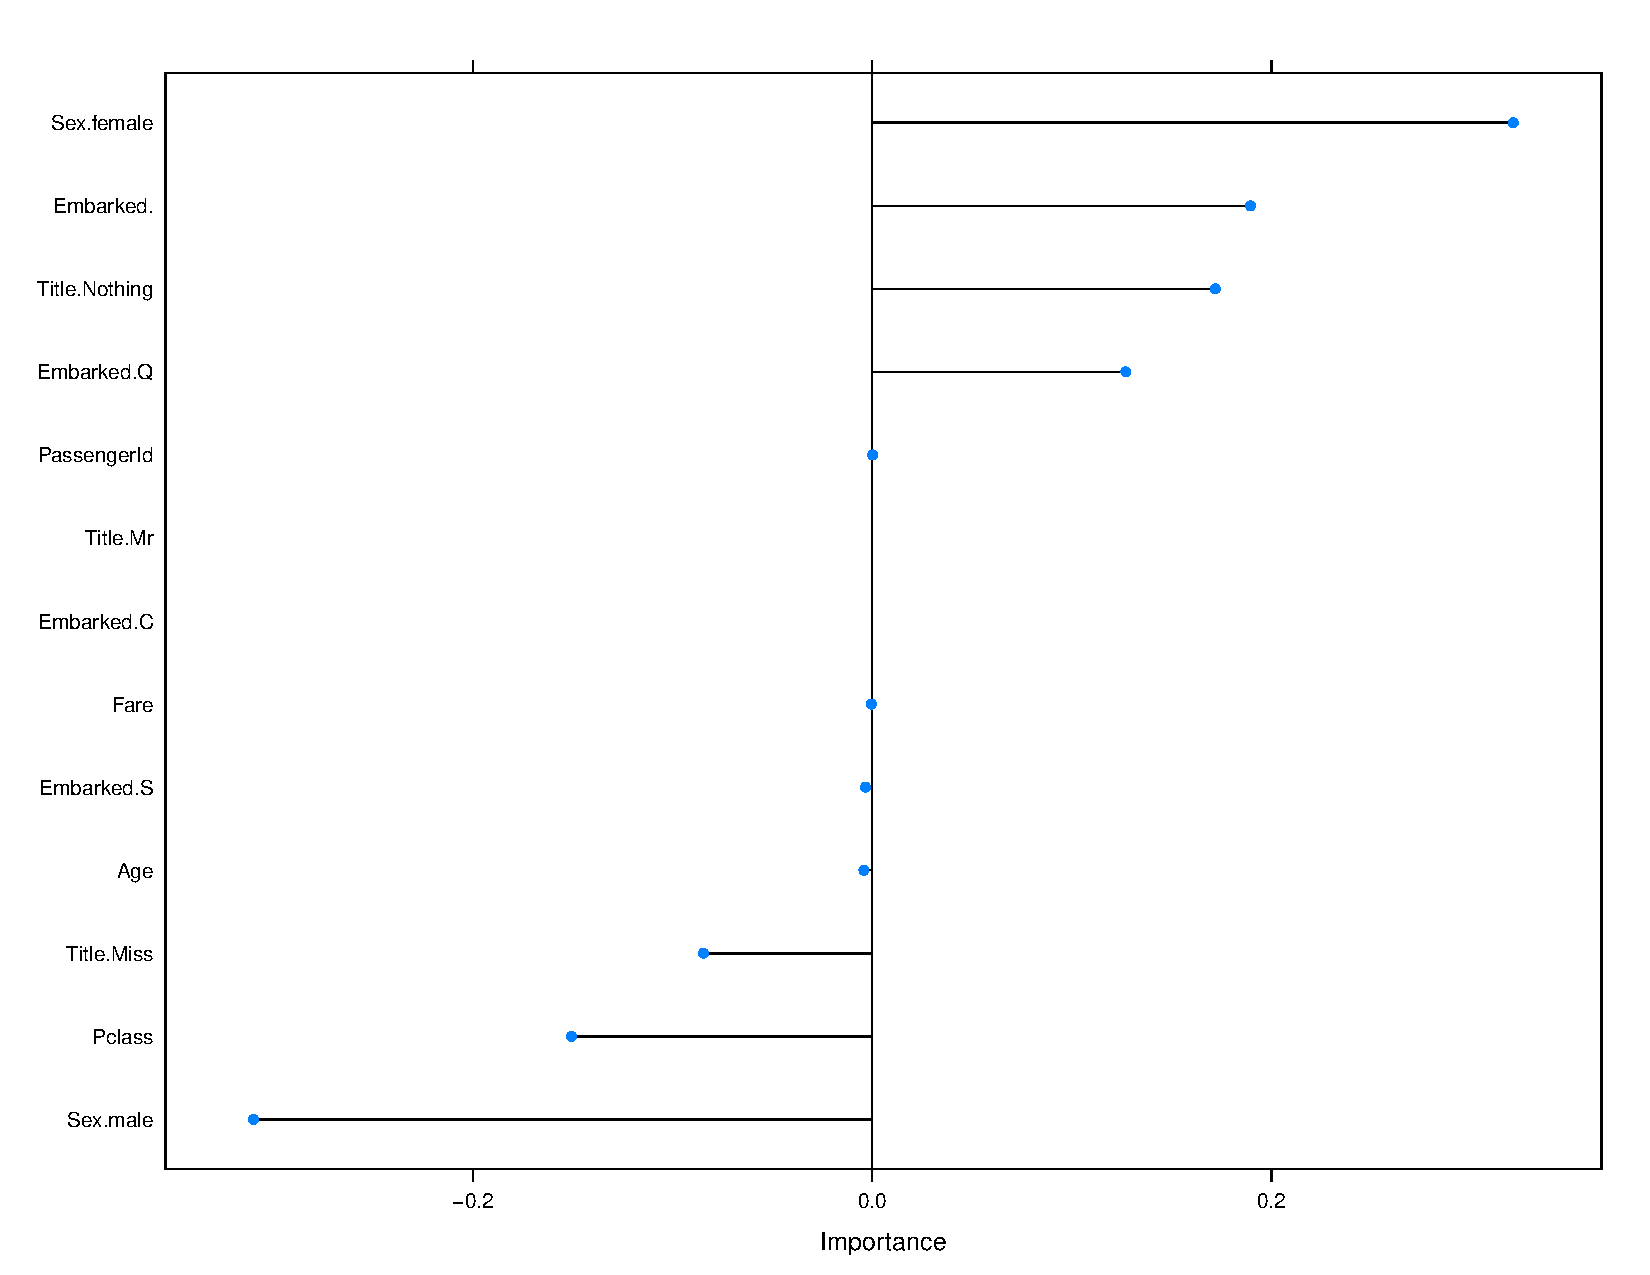
\includegraphics[page=1,width=6.5 in]{Rplot02.pdf}}

The bar chart shows the positive/negative significance of the parameters. Apparently, sex is the most important factor that predicts the survival rate, females has higher rate of survival. Followed by the embark station, title, Pclass, etc. Surprisingly, fare and age are not important factors. 

\begin{verbatim}
> predictions <- predict (object = objModel, testTitanic[, predictorNames])
> auc <- roc(testTitanic[,outcomeName], predictions)
> print(auc$auc)
Area under the curve: 0.8162

glmnet 

643 samples
 14 predictor

No pre-processing
Resampling: Bootstrapped (25 reps) 
Summary of sample sizes: 643, 643, 643, 643, 643, 643, ... 
Resampling results across tuning parameters:

  alpha  lambda        RMSE       Rsquared   RMSE SD     Rsquared SD
  0.10   0.0005830662  0.3765114  0.4104477  0.01630625  0.04802805 
  0.10   0.0058306620  0.3764802  0.4104577  0.01627727  0.04815431 
  0.10   0.0583066196  0.3773712  0.4082301  0.01583780  0.05017336 
  0.55   0.0005830662  0.3765384  0.4103637  0.01630760  0.04799849 
  0.55   0.0058306620  0.3766363  0.4098028  0.01620765  0.04849452 
  0.55   0.0583066196  0.3839395  0.3926058  0.01424758  0.05105830 
  1.00   0.0005830662  0.3765460  0.4103390  0.01630296  0.04801072 
  1.00   0.0058306620  0.3769947  0.4086266  0.01617720  0.04899620 
  1.00   0.0583066196  0.3902637  0.3812531  0.01328293  0.05424078 

RMSE was used to select the optimal model using  the smallest value.
The final values used for the model were alpha = 0.1 and lambda = 0.005830662. 
\end{verbatim}
The auc scour is 0.8162 (0.5 auc score is random and 1 is perfect). Final values for model parameters  are alpha $=$ 0.1 and lambda $=$ 0.005830662. 


\end{document}